\section{Application}
For a given island, a particular bait density is required on the ground for a successful rodent eradication. This density is determined after studying the ecosystems of the island and the biology of the invasive target species. Given the required bait density and the total area of the island, the minimum amount of bait needed for the eradication operation can be calculated using NERD. While planning helicopter flights paths, it is assumed that the bait density within each swath is constant, but variable between swaths.

Assuming a variable bait density along each swath but uniform density across the
swath, we can estimate bait density with greater precision after the aerial
dispersal given that the bait density for each cell is calculated between two consecutive points recorded by the GPS. This case considers the effects on
density when the helicopter flies with variable speed (Figure \ref{fig:densidadSimetrica}).

To account for the well known fact that we have a higher density of rodenticide right bellow of the helicopter and lower densities along the edges of the swath, we can assume a variable bait density both along and across each swath.  This allows for the detection of areas where the bait density is below the lower limit of the target bait density or of gaps on the ground without any bait (Figure \ref{fig:densidadSimetrica}).

\begin{figure}
  \centering
  \begin{subfigure}[b]{0.45\textwidth}
    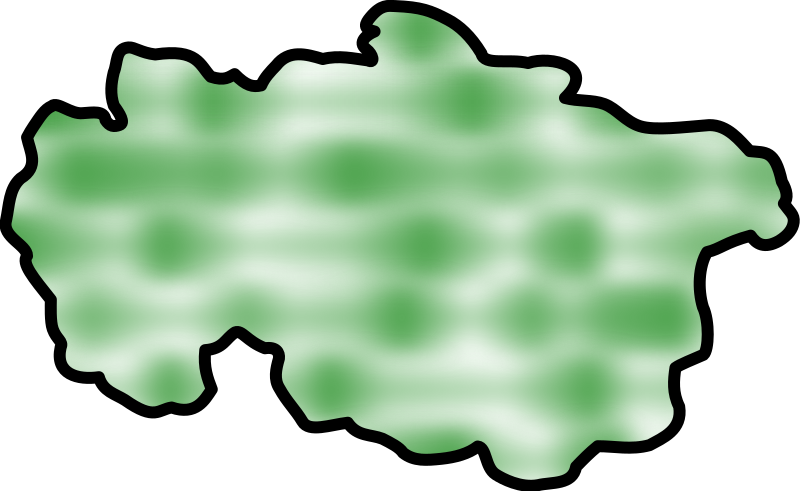
\includegraphics[width=\textwidth]{../resultados/png/symmetric-bait-density.png}
    \caption{
    Symmetric bait density
    }
    \label{fig:densidadSimetrica}
  \end{subfigure}
  \begin{subfigure}[b]{0.45\textwidth}
    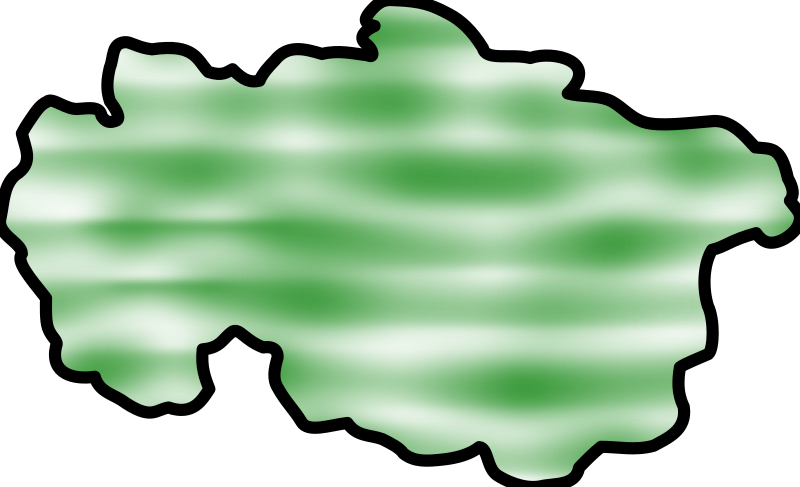
\includegraphics[width=\textwidth]{../resultados/png/asymmetric-bait-density.png}
    \caption{
    Asymmetric bait density
    }
    \label{fig:densidadAsimetrica}
  \end{subfigure}
  \caption{
  \ref{fig:densidadSimetrica}
  Hypothetical island with symmetric variable bait density across each swath.
  \ref{fig:densidadAsimetrica}
  Hypothetical island with asymmetric variable bait density across each swath.}
\end{figure}

To account for the effect of the wind on the bait density profile, an asymmetric
and fully variable bait density distribution within each swath is allowed
(Figure \ref{fig:densidadAsimetrica}).
